\documentclass[letterpaper,12pt]{book}

\usepackage{amsmath}
\usepackage[utf8]{inputenc}
\usepackage[spanish]{babel}
\usepackage{graphicx}
\usepackage[normalem]{ulem}
\usepackage[backend=biber]{biblatex}
\usepackage{hyperref}
\usepackage{amssymb}
\usepackage[Sonny]{fncychap}
\usepackage{blindtext} %% TO BE REMOVED

\addbibresource{references.bib}
\graphicspath{ {images/} }

\begin{document}
\frontmatter
    \thispagestyle{empty}
\begin{minipage}{.3\textwidth}
  \flushleft
  \center{
\includegraphics[scale=.09]{unam}}

  \vspace{20pt}

  \center{
    \rule{.5pt}{.6\textheight}
    \hspace{7pt}
    \rule{2pt}{.6\textheight}
    \hspace{7pt}
    \rule{.5pt}{.6\textheight}
  } \\

  \center{
\includegraphics[scale=.22]{ciencias}}
\end{minipage}
\begin{minipage}{.7\textwidth}
\flushright

\center{

  \center{
    \LARGE{U}\large{NIVERSIDAD} \LARGE{N}\large{ACIONAL}
    \LARGE{A}\large{UTÓNOMA} \\[10pt]
    \large{DE}
    \LARGE{M}\large{ÉXICO}
  } \\
  \rule{\textwidth}{2pt}
  \\
  \hrulefill\\[1cm]

  \LARGE{F}\large{ACULTAD DE } \LARGE{C}\large{IENCIAS}\\[2cm]

  \large{
Implementación de redes neuronales convolucionales para el estudio de interacciones proteina-ligando  }\\[2cm]

  \huge{
T \hspace{1cm} E \hspace{1cm} S \hspace{1cm} I \hspace{1cm} S  }\\[1cm]

  \large{QUE PARA OBTENER EL TÍTULO DE:}\\[1cm]

  \large{
Matemático  }\\[1cm]

  \large{PRESENTA:}\\[1cm]

  \large{
Adrián Antonio Rodríguez Pié  }\\[1cm]

  \large{
TUTOR  }\\[1cm]

  \large{
Marcelino Arciniega Castro  }
}\\
  \large{
Ciudad Universitaria, CDMX, 2019
}

\end{minipage}

    \tableofcontents
    \section{Abstract}
El descubrimiento de nuevos fármacos es un proceso muy tardado y costoso.
El desarrollo e incluso el reposicionamiento de compuestos ya conocidos es una
tarea sumamente complicada. El escenario es aún más complicado si se toman en cuenta
los miles o millones de moléculas capáces de ser sintetizadas en cada etapa del desarrollo.
Para superar estas dificultades, el uso de alternativas computacionales de bajo costo
es altamente recomendado, y se ha adoptado como la forma estándar te ayuda para el
desarrollo de nuevos fármacos.

Una de las metodologias computacionales más usades para investigar estas interacciones es
el acoplamiento molecular. La selección de los ligandos más potentes utilizando Cribado
Virtual basado en Acoplamiento (DBVS) es realizado a través de realizar la inserción de
cada compuesto de la bibilioteca de compuestos en una región particular de un receptor
objetivo. En la primera etapa del proceso, una búsqueda heurística es llevada a cabo
en la que miles de posibles inserciones son consideradas. En la segunda etapa, la calidad
de la inserción es evaluada a través de una función evaluadora. Esta última fase se ha
convertido en todo un reto para los científicos computacionales, por la dificultad de decidir
de forma determinística si un acoplamiento es bueno o no.

Los sistemas basados en aprendizaje de máquina (ML) han sido usados con éxito para mejorar la
salida del DBVS para tanto incrementar el desempeño de las funciones evaluadoras, como para
construir clasificadores de afinidad de enlace. Una de las principales ventajas de utilizar ML
es la capacidad de explicar la dependencia no lineal de las interacciones moleculares entre
ligando y receptor.

En este trabajo se propone un acercamiento con una red neuronal convolucional para mejorar el
DBVS. El método utiliza los resultados de una simulación de acoplamiento como entrada, en
donde automáticamente aprende a extraer características relevantes a partir de datos básicos
como tipos de átomo, distancias entre ellos, y su contexto en la rama estructural. La red
aprende características abstractas que son útiles para discriminar entre ligandos activos y
señuelos en una proteína.


\mainmatter
    \chapter{Marco teorico}
        Un factor que ha sido central en la historia del ser humano es
precisamente el que nos da el nombre como especie \textit{Homo
sapiens}: la inteligencia. Durante años se ha buscado entender cómo es
que pensamos; es decir, la forma en que un ente puede percibir el
entorno y, a partir de ello, entenderlo e incluso manipularlo y hacer
predicciones al respecto.  La inteligencia artificial (IA) lleva este
estudio un paso más adelante: busca no sólo entender sino también
construir entes inteligentes.

\section{La prueba de Turing}
Dado que la inteligencia artificial busca crear entes inteligentes,
es importante definir primero qué es la inteligencia. Al ser nosotros
mismos como especie nuestro modelo de inteligencia, es razonable pensar
en la inteligencia en términos de pensamiento humano.

La \textbf{prueba de Turing}, propuesta por Alan Turing (1950), fue
diseñada para dar una definición de inteligencia en computadoras. Una
computadora pasa la prueba si, tras ser interrogada de forma escrita
por un evaluador humano, éste no puede distinguir si las respuestas
provienen de un humano o una computadora.  La discusión sobre si pasar
la prueba realmente es señal de una \textit{inteligencia} sale del
alcance de esta tesis, pero es importante resaltar que la prueba da
cierta noción sobre lo que se busca en una ``inteligencia
artificial''.  Se busca que el ente ``inteligente'' sea capaz de tener
un criterio racional.  Es decir, que pueda sacar conclusiones lógicas
a partir de premisas dadas mediante silogismos, como lo haría un
humano. Pero rara vez toda la información con la que se cuenta es
100\% acertada, lo que echa abajo el enfoque puramente determinista de
la inteligencia.

\section{Agentes}
En su concepción más tradicional, la inteligencia artificial gira en torno a
\textbf{agentes racionales} que, mediante \textbf{sensores} pueden percibir
su \textbf{entorno} y actuar sobre él a partir de un sistema de
decisión.  Internamente, el agente es una máquina compuesta por un
conjunto (finito) de estados, cuyas transiciones están dadas por
reglas de inferencias. Cuando se da una transición de estados,
entonces es ejecutada una acción. Esta concepción del agente nos
permite reducir la IA a un problema de búsqueda de las funciones de
transición.

Computacionalmente hablando, la búsqueda de estas funciones en ciertos
problemas de IA se vuelve absurdamente compleja, por lo que no es
factible hacer la codificación de todos los posibles escenarios en el
sistema de inferencia de un agente. Por lo tanto, un agente debe ser
capaz de manejar la incertidumbre en su entorno. Además, debe
poder \textit{aprender} del entorno y adaptarse a él, generando
conocimiento por medio de la experiencia.

El \textbf{aprendizaje de máquina} (ML, \textit{Machine Learning})
gira en torno a algorítmos capaces de manejar información estocástica
y generar modelos de toma de decisiones a partir de ella. \textbf{Un
modelo es bueno en la medida de lo acertado que es en términos
estadísticos}.

\section{Tipos de aprendizaje}
El aprendizaje de máquina se ha divido en varios subcampos, cada uno
atacando un tipo de problema distinto y utilizando diferentes formas
de aprendizaje. Se describen a continuación cuatro parámetros bajo
los cuales es posible clasificar los distintos paradigmas de
aprendizaje.\\

\textbf{Supervisado/no supervisado.} Dado que el aprendizaje involucra
una interacción entre el agente y el ambiente, es posible
dividir el aprendizaje con respecto a la naturaleza de dicha interacción.
La primera distinción a notar es la diferencia entre aprendizaje supervisado
y no supervisado. En abstracto, viendo el aprendizaje como un proceso
de ``usar la experiencia para ganar \textit{maestría}'', el aprendizaje
supervisado describe un escenario en el que la ``experiencia'', un
ejemplo de entrenamiento, contiene información significativa que no
está contenida en los ``ejemplos de prueba'' que el sistema aún no ha
visto, y en los que se busca aplicar la \textit{maestría} adquirida.
En esta configuración, la \textit{maestría} adquirida busca
predecir la información faltante de los datos de prueba. Podemos
pensar en el ambiente como un profesor que ``supervisa'' al agente
al proporcionarle información extra (una clasificación). Por otro lado,
en el aprendizaje no supervisado no hay distinción entre datos de
entrenamiento y de prueba. El agente procesa los datos de entrada
con el objetivo de generar una síntesis o versión comprimida de los
datos que sea representativa.\\

\textbf{Agentes pasivos/activos.} En los paradigmas de aprendizaje
el rol tomado por el agente varia. Es posible distinguir entre
agente activo y pasivo. Un agente activo interactúa
con el ambiente durante el entrenamiento, haciendo consultas o
experimentos, mientras que un agente pasivo sólo observa la
información provista por el ambiente sin influir
o dirigirla durante el proceso de aprendizaje.\\

\textbf{Ayuda del profesor.} Cuando se piensa en el aprendizaje humano
el proceso, por lo general, involucra a un profesor que está tratando
activamente de proveer al agente con la información más útil para
lograr el objetivo de aprendizaje. En contraste, cuando un científico
aprende sobre la naturaleza o el ambiente, tomando el rol de profesor,
puede ser pensado como pasivo: las manzanas caen, las estrellas
brillan y la lluvia cae sin cuidado por el aprendizaje del agente.
Dichos escenarios son modelados postulando que los datos de
aprendizaje (o la experiencia del agente) son generados por un proceso
aleatorio.\\

\textbf{Protocolo de entrenamiento lineal (o en línea)/por lote.} El
último parámetro a mencionar es la distinción entre las situaciones en
las que el agente tiene que responder de forma lineal; es decir, que
para cada ejemplo de entrenamiento tiene que dar una respuesta, y
el agente tiene que mostrar el aprendizaje adquirido después de
tener la oportunidad de procesar grandes cantidades de datos.

        \section{Sobre compuertas y neuronas}
Los modelos de redes neuronales artificiales, uno de los cuales es el \textit{perceptrón}
que discutiremos en este capitulo, están inspirados en el cerebro humano. Hay científicos
cognitivos y de neurociencia cuya meta es entender el funcionamiento del cerebro, y con
esto en mente, construir modelos de las redes neuronales naturales del cerebro.

Sin embargo, lo que busca la inteligencia artificial es construir máquinas \textit{útiles}
tomando como modelo el cerebro. El cerebro es un dispositivo de procesamiento de información
con habilidades asombrosas en muchos campos que sobrepasan con creces a los más grandes
esfuerzos de la ingenieria, como son visión, aprendizaje y reconocimiento del habla, por
nombrar algunos.
\subsection{Inspiracion en la biología}
El cerebro humano es muy diferente de una computadora. Mientras una computadora tiene
un número reducido de procesadores, el cerebro está compuesto de una enorme cantidad $(10^{11})$
de unidades de procesamiento llamadas \textbf{neuronas} trabajando en paralelo.

Aunque los detalles son inciertos, se cree que las neuronas son mucho más simples y lentas
que un procesador de una computadora \cite{ethem}. Lo que hace al cerebro distinto, y le da
su gran poder computacional, es su gran conectividad: las neuronas en el cerebro tienen
conecciones, llamadas \textit{sinápsis}, a alrededor de otras $10^{4}$ neuronas.

En una computadora, el procesador es activo y la memoria está separada y opera de forma pasiva
(el procesador accede a ella sólo cuando se requiere); se cree que en el cerebro, tanto el
procesamiento como la memoria están distribuidos por toda la red. El procesamiento es realizado
por las neuronas y la memoria se encuentra en las sinápsis entre ellas.

El cerebro es, además, un órgano capás de adaptarse a las condiciones de su ambiente, ya que
constantemente son agregadas nuevas conexiones sinápticas entre neuronas y modificadas
las ya existentes. Una vez que una neuroan ha emitido una señal eléctrica, las adyacentes
reciben la información por medio de canales de transmisión llamados \textit{dendritas}. Estos
impulsos son llevados hasta el \textit{núcleo} de la neurona para su procesamiento y, posteriormente,
una reacción es transmitida a través del \textit{axón} de la célula \cite{memes}.

\textbf{Imagén de https://psi121f.wordpress.com/2016/07/03/la-estructura-de-la-neurona-2/}



\section{Perceptron}
En 1943, Warren McCullock y Walter Pitts publican la primera aproximación de una
neurona simplificada, tratando de entender cómo funciona el cerebro biológico para
el dieseño de inteligencia artificial, la llamada neurona McCullock-Pits (MCP) \cite{mcp}.

McCullock y Pitts describen a la neurona como una compuerta lógica sencilla con una
salida binaria; múltiples señales llegan a las dendritas para ser integradas al cuerpo
de la célula. Si la señal acumulada excede cierto umbral, se genera una señal de salida
que se le pasa al axón.

Unos años después, Frank Rosenblatt publica la primera aproximación al concepto de
perceptron basado en el modelo de neuronas MCP \cite{rosenblatt}. Intuitivamente, el algoritmo
aprende automáticamente los coeficientes de pesos óptimos que luego se multiplican
con las características de entrada para tomar la decisión de si la neurona se activa
o no. Este algoritmo podría ser usado entonces para predecir si una muestra pertenece
a una clase o a otra \cite{python}.

Formalmente, podemos plantearlo como un problema de clasificación binaria, donde nos
referimos a nuestras dos clases, por simplicidad, como 1 (clase positiva) y -1
(clase negativa). Definimos también una \textit{función de activación $\mathbf{\phi (z)}$}
que toma una combinación lineal de ciertos valores de entrada \textbf{x} y un
vector de pesos \textbf{w}, donde \textbf{z} es la llamada \textit{entrada de la red}
$(z = w_1x_1 + ... + w_mx_m)$:

\begin{equation*}
w=
    \begin{bmatrix}
        w_1 \\
        \vdots \\
        w_m
    \end{bmatrix}
    , x=
    \begin{bmatrix}
      x_1 \\
      \vdots \\
      x_m
    \end{bmatrix}
\end{equation*}
\\
Si la activación de una muestra particular $x^{(i)}$ es mayor que un parámetro definido
$\theta$, predecimos la clase 1, y la clase -1 en caso contrario. En el algoritmo
del perceptrón de Rosenblatt, la activación de función $\phi (\dot)$ es una \textit{función escalón},
que es llamada a veces la \textit{función de Heaviside}:
\begin{equation*}
  \phi(z)= \left\{ \begin{array} {rl}
    1 & \text{si } z \geq \theta \\
    -1 & \text{en otro caso} \end{array} \right.
\end{equation*}

Por simplicidad, definimos $w_0=-\theta$ y $x_0=1$, escribiendo entonces a $z$ de la
forma $z=w_0x_0 + w_1x_1 + \dots + w_mx_m = \mathbf{w^Tx}$.
La siguiente imágen ilustra cómo la entrada de la red $z=w^Tx$ es \textit{aplanada}
a una salida binaria (-1 o 1) por la función de activación del perceptrón (izquierda)
y cómo puede ser usada para discriminar entre dos clases linealmente separables (derecha):
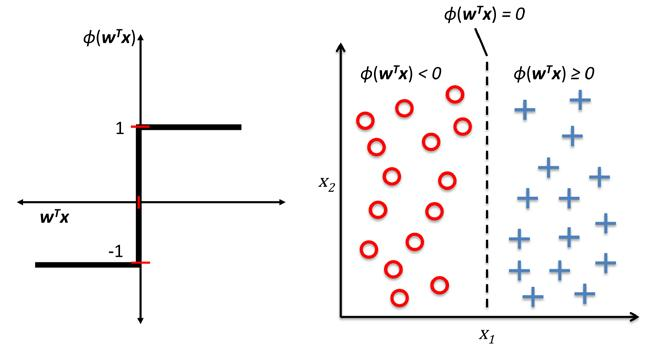
\includegraphics[scale=0.5]{perceptron}\cite{python}

La idea detrás del modelo de perceptron de Rosenblatt es reducir a una abstracción de cómo funciona
una neurona: se activa o no se activa. Así, la regla inicial de Roseblatt es relativamente
simple y puede ser resumida en los siguientes pasos:

1. Inicializar los pesos en cero o en números aleatorios cercanos a cero.

2. Para cada muestra de entrenamiento $x^{(i)}$ realizar los siguientes pasos:

1. Caluclar el valor de salida $\hat y$.
2. Actualizar los pesos.


En este caso, el valor de salida es la clasificación dada por la función escalón
definida previamente, y la actualización simultánea de cada peso $w_j$ en el
vector de pesos $w$ puede ser escrito más formalmente cómo:
\begin{equation}
  w_j := w_j + \Delta w_j
\end{equation}

El valor de $\Delta w_j$, que es usado para actualizar el peso $w_j$, es
calculado por la regla de aprendizaje de percetron:
\begin{equation}
  \Delta w_j = \eta (y^{(i)} - \hat y^{(i)})x^{(i)}_j
\end{equation}

Donde $\eta$ es el índice de aprendizaje (una constante entre 0 y 1),
$y^{(i)}$ es la clasificación real de la i-ésima muestra, y $\hat y^{(i)}$
es la clasificación dada por la predicción. Es importante recalcar que
todos los pesos en el vector de pesos son actualizados de manera
simultánea, lo que significa que no recalculamos $\hat y^{(i)}$ hasta que
todos los pesos $\Delta w_j$ han sido actualizados.

Podemos resumir el concepto general de perceptron con la siguiente imágen:
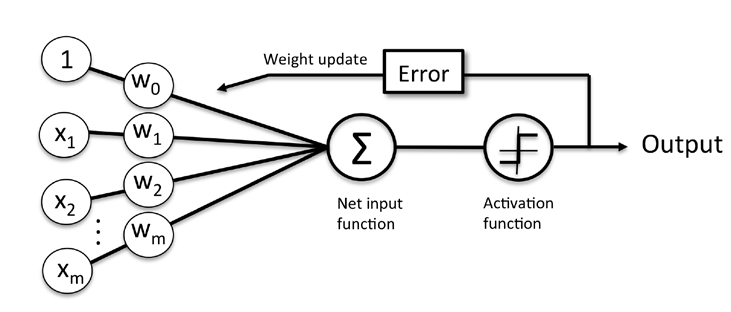
\includegraphics[scale=0.5]{perceptron-summary}\cite{python}

La imágen anterior muestra cómo el perceptron recibe las entradas de una
muestra $x$ y las combina con los pesos $w$ para calcular la entrada neta.
Esta entrada se le dá a la función de activación, que genera una salida
binaria (-1 o 1 en este caso), representando la predicción de la clasifica-
ción. Durante la fase de aprendizaje, la salida es usada para calcular el
error de la predicción y actualizar los pesos.

        \section{Capítulo sin nombre}
\subsection{Descenso por el gradiente}
Uno de los puntos clave del aprendizaje de máquina supervisado es
definir una función objetivo que deberá ser optimizada durante el
proceso de aprendizaje. Esta función objetivo usualmente es una
\textbf{función de costo, pérdida o error} que se quiere minimizar.

La no-linealidad de las funciones de activación provocan que no se garantice la convexidad
de las funciones de error más comunes, es decir, que no existe un método analítico para
encontrar el mínimo de la función de error, el entrenamiento de la red se basa en
métodos iterativos que van reduciendo paulatinamente ese error. 

Definimos la función de costo $J$ como la \textbf{Suma de
  los errores cuadrados (SSE)} entre la salida calculada y el valor
real.
\begin{equation}
  J(w)=1/2n \sum_i (\hat{y}_i - y_i^2)
\end{equation}
donde $w$ es el conjunto de los parámteros de la red, es decir
$w := \bigcup{W_i, b_i}_{i=1}^{n}$, $n$ el número de capas de la red, y $y_i$
la $i$-ésima etiqueta de entrenamiento.

La principal ventaja de esta función de error, además de ser lineal
es que la función de costos se vuelve diferenciable.

Sabemos que la derivada es útil para minimizar funciones porque, dada una función
$y = f(x)$, nos dice cómo cambiar $x$ para hacer una pequeña mejora en $y$, en
otras palabras $f(x-\varepsilon f'(x)) < f(x)$ para un $\varepsilon \epsilon \mathbb{R}$
suficientemente pequeño. Podemos entonces reducir $f(x)$ al mover a $x$ en pequeños
\textit{pasos} con el signo opuesto de la derivada. A esta técnica se le conoce como
\textbf{descenso por el gradiente}.

La idea detrás del descenso por el gradiente es disminuir el gradiente hasta encontrar
un mínimo (local o global) de la función de costo. En cada iteración, se reduce
un \textit{paso} del gradiente, donde cada \textit{paso} está determinado por
el valor del índice de aprendizaje, así como por la pendiente del gradiente.

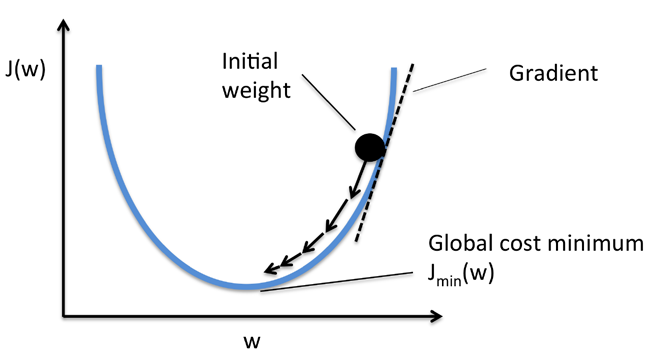
\includegraphics[scale=0.5]{gradient-descent}

Usando el descenso por el gradiente, se pueden actualizar los pesos quitandole un \textit{paso}
al gradiente $\nabla J(w)$ de la función de costos $J(w)$:
\begin{equation}
  w := w + \Delta w
\end{equation}

En donde el cambio de peso $\Delta w$ se define como el gradiente negativo multiplicado
por el índice de aprendizaje $\eta$:
\begin{equation}
  \Delta w := -\eta \Delta J(w)
\end{equation}

Calculamos la derivada parcial de la función de costos SSE con respecto al
j-ésimo peso de la siguiente manera:
\begin{equation*}
\begin{split}
  \frac{\partial J}{\partial w_j} &= \frac{\partial}{\partial w_j}\frac{1}{2}\sum_i (y^{(i)} - \phi(z^{(i)}))^2 \\
  &= \frac{1}{2}\sum_i 2(y^{(i)} - \phi(z^{(i)}))\frac{\partial}{\partial w_j}(y^{(i)} - \phi(z^{(i)}))\\
  &= \sum_i (y^{(i)} - \phi(z^{(i)}))\frac{\partial}{\partial w_j}(y^{(i)} - \phi (z^{(i)}))\\
  &= \sum_i(y^{(i)} - \phi(z^{(i)}))(-x_j^{(i)})\\
  &= -\sum_i(y^{(i)} - \phi(z^{(i)}))x_j^{(i)}
\end{split}
\end{equation*}

\subsection{Propagación hacia atrás}
FALTA SECCIÓN
\cite{haykin} 129
\cite{memes} 36
http://www.iro.umontreal.ca/~pift6266/H10/notes/mlp.html

\subsection{Convolución}
FALTA SECCIÓN

        Las proteínas son macromoléculas formadas por cadenas lineales de
aminoácidos, cada una de las cuales se denomina polipéptido. El
término \textbf{proteína} se origina del griego \textit{proteios} que
significa ``primario'' o ``de primer orden''. El nombre fue adoptado
por Jöns Berzelius en 1838 para enfatizar la importancia de esta clase
de moléculas. Las proteínas juegan un rol crucial en el mantenimiento
de la vida, ya que son el soporte para la arquitectura del tejido
muscular, ligamentos, tendones, huesos, piel, cabello, órganos y
glándulas. Proveen los servicios fundamentales de transporte y
almacenamiento como en el caso del oxígeno y hierro en células
musculares y eritrocitos. También participan en muchos procesos
regulatorios esenciales, como reacciones de catálisis, funciones
inmunológicas y hormonales, así como en la coordinación de actividades
neuronales y diferenciación celular.\cite{tamar}

\begin{figure}[H]
  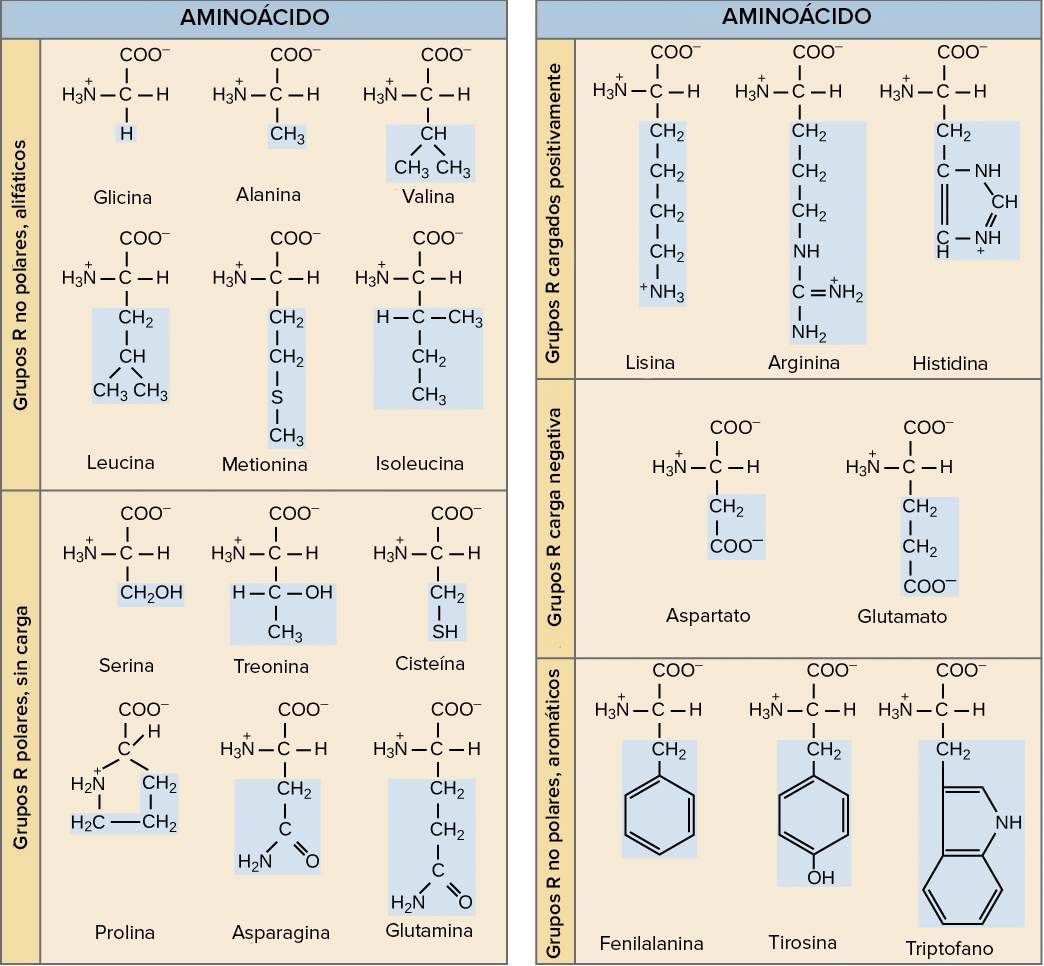
\includegraphics[scale=0.3]{aminoacids} \centering
  \caption{Existen sólo 20 tipos de aminoácidos en las proteínas
  (Tomado de \url{https://cnx.org/contents/GFy_h8cu@11.9:2zzm1QG9})}
\end{figure}

\section{Ligandos}
La comunicación entre moléculas es dada por medio de señales químicas.
Estas señales químicas son mandadas en forma de moléculas pequeñas,
usualmente volátiles o solubles, llamadas ligandos.
Un \textbf{ligando} es una molécula que se une a otra molécula
específica, en algunos casos, mandando una señal el proceso. Los
ligandos interactuan con proteínas en células objetivos.  Son a estas
proteínas a las que llamamos \textbf{receptores}. Estas interacciones
con el receptor se dan en áreas específicas de la estructura, a las
que comunmente se les conoce como \textbf{sitios activos}.

Las interacciones proteína-ligando y proteína-proteína juegan un papel
fundamental en el descubrimiento de fármacos. Es por eso que se han
desarrollado una variedad de metodologías para investigar dichas
interacciones. En este trabajo nos enfocamos en el acoplamiento
molecular.

\section{Acoplamiento molecular}
El campo del \textbf{acoplamiento molecular} o
\textbf{docking} surge a lo largo de las últimas tres décadas gracias a la
necesidad de la biología molecular en cuanto al descubrimiento de
inhibidores basado en estructuras. Ha podido evolucionar
considerablemente gracias al crecimiento dramático de disponibilidad y
poder de las computadoras, y al creciente acceso a bases de datos de
proteínas y moléculas.\cite{kukol}

\begin{figure}[H]
  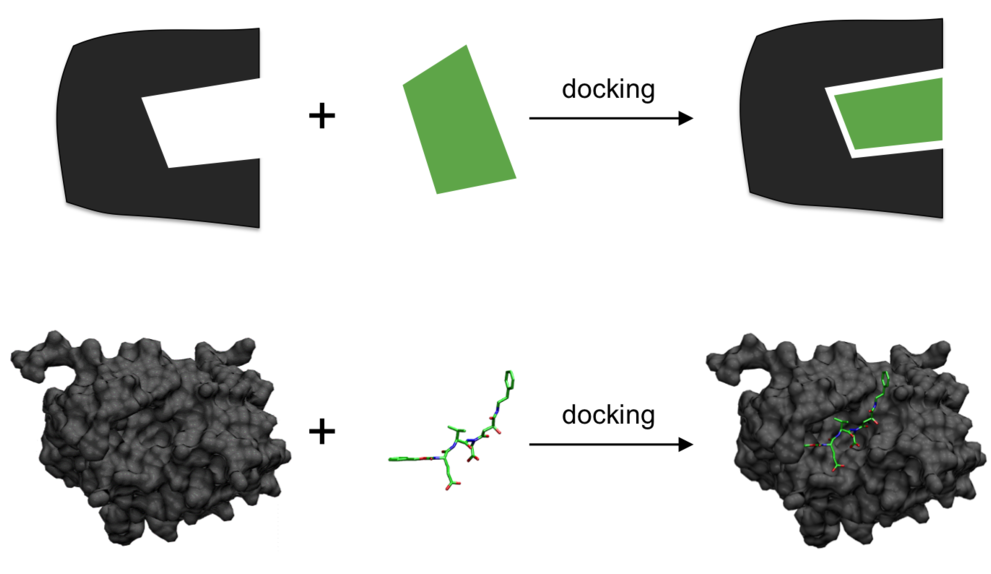
\includegraphics[scale=0.3]{docking} \centering
  \caption{Representación esquemática del \textit{docking}.  (Tomado de
    \url{https://en.wikipedia.org/wiki/Docking_(molecular)})}
\end{figure}

El objetivo de un programa de acoplamiento molecular automatizado es comprender
y predecir reconocimiento molecular, tanto estructuralmente, encontrando
posibles \textit{poses} de acoplamiento, como energéticamente, prediciendo la
afinidad del enlace. El acoplamiento molecular usualmente se realiza entre una
molécula pequeña, un ligando, y una macromolécula objetivo, una proteína en
nuestro caso.

\begin{figure}[H]
  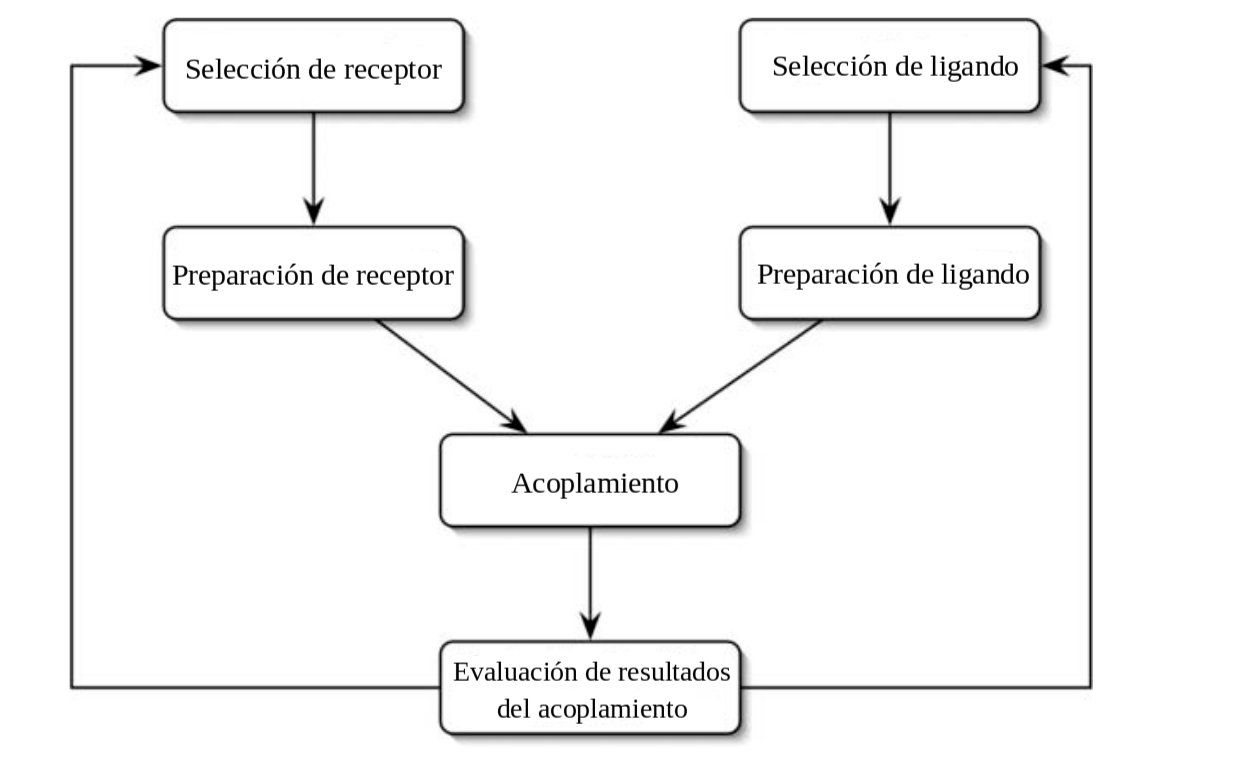
\includegraphics[scale=0.5]{docking_steps}
  \caption{Diagrama de flujo para un acoplamiento usual.  (Tomado de
    \cite{kukol})}
  \label{fig:docking_flowchart}
\end{figure}

La figura \ref{fig:docking_flowchart} muestra los pasos clave que son
comunes en todos los protocolos. El acoplamiento consiste en encontrar
las poses de unión más favorables de un ligando hacia una proteína
objetivo. La pose de unión de un ligando puede ser caracterizado de
forma única por sus variables de estado. Éstas consisten en su
posición (traslaciones sobre los ejes $x, y, z$), orientación (ángulos
de Euler o cuaterniones) y, si el ligando es flexible, su conformación
(los ángulos de torsión para cada enlace de rotación). Cada una de las
variables de estado describe un grado de libertad en un espacio de
búsqueda multidimensional.

\section{Función evaluadora}
Todos los métodos de acoplamiento requieren una función de evaluación
para calificar las poses de unión de los candidatos, y un método de
búsqueda para explorar las configuraciones de las variables de
estado. En general, el éxito de un acoplamiento se mide en términos de
la \textit{desviación media cuadrática} (RMSD, \textit{Root-mean-
square deviation}) de las coordenadas cartesianas de los átomos del
ligando en las conformaciones del acoplamiento, comparadas con las
cristalográficas. Un acoplamiento se considera exitoso si el RMSD es
menor a 2\AA.

\section{Archivos PDB}
El banco de datos de proteínas es un archivo de estructuras de
macromoléculas biológicas determinadas experimentalmente. El formato
utilizado para almacenar está información contiene elementos como
coordenadas de átomos, nombres de moléculas e información sobre
estructuras primarias y secundarias. Es con este formato con el que se
trabajó durante el proyecto.
\footnote{\url{ftp://ftp.wwpdb.org/pub/pdb/doc/format_descriptions/Format_v33_Letter.pdf}}

\section{SMILES}
SMILES (\textit{Simple Molecular Input Line Entry System}) es un
sencillo lenguaje químico que permite describir moléculas y reacciones
utilizando únicamente caracteres ASCII que representan símbolos de
átomos y enlaces. Una cadena SMILES contiene la misma información que
una tabla de conexiones extendida, pero con varias ventajas: es
sumamente compacta y puede ser canonizada de tal manera que puede ser
usada como identificador universal para una estructura química
dada.\footnote{\url{http://www.daylight.com/smiles/}}

    \chapter{Metaanálisis del acoplamiento}
        \section{Workflow}
\subsection{¿Qué se hizo?}
Se tomó una base de datos cristalográfica de acoplamientos ya
realizados y sobre esos ligandos y proteinas se corrió Docking con
AutoDockVina n.m. Después se hace una tabla comparando los scores que
les asigna AutoDockVina con el RMSDI cristalográfico. Pero los scores
de autodockvina no siempre son muy buenos y pasa que muchas veces la
que es la mejor pose la manda al $4^o$ o $5^o$ lugar del ranking.
Aquí es donde entra la red:

Pereira, Caffaren y dos Santos \cite{dossantos} consideran al átomo
como una entidad ligada íntimamente con su contexto. Con esta premisa,
crean una red que toma como entrada a cada átomo del ligando con su
contexto codificado, entendiendo contexto del átomo como las
carácteristicas de este y de los átomos más cercanos.
Pereira buscaba encontrar el acoplamiento que generara la mayor
cantidad de energía, sin importar cual fuera la conformación necesaria
para poder realizarlo; nuestro enfoque busca precisamente encontrar
dicha conformación.

\subsubsection{Contexto de la rama}
Partiendo de la ídea del átomo ligado a su contexto, y considerando
que lo que buscamos encontrar es una propiedad puramente estructural,
tomamos como unidad básica del ligando a la rama. Así, nuestro
\textit{contexto de átomo} se convierte en \textbf{contexto de rama},
siendo este la combinación de el tipo de rama, los de las ramas más
cercanas y la distancia a cada una de ellas.

A partir de ese diccionario (con su respectivo índice), se asocia a
una rama con las cinco ramas más cercanas codificadas a través de sus
tipos y sus distancias a las ramas dadas. Esto se hace para cada rama
del ligando.

Para el tipo de rama se divide cada ligando en sus respectivas ramas y
cada una de estas ramas se codifica usando la respresentación
SMILES \footnote{\url{http://www.daylight.com/smiles/}} y se ponen en
un listado donde se asocia cada rama codificada con un índice,
generando así lo que llamamos el \textit{diccionario de ramas}.

Luego, una capa convolucional es empleada para sintetizar la
información de todos los contextos de todas las ramas del ligando y
genera una representación vectorial del complejo. Después se pasa a
dos capas ocultas para sintetización y procesamiento del
vector-ligando. Finalmente, en la última capa, la representación del
complejo es dada como entrada a un clasificador \textit{softmax},
quien es responsable de producir el puntaje. A continuación se
presenta un pseudo-código de alto nivel del proceso de la red:
\begin{algorithm}
  \caption{Deep-pose}
  \begin{algorithmic}[1]
    \State \textbf{Dados:}\newline
                           $W_{b\_type} \in \mathbb{R}^{h\times |B|}, W_{b\_dist}
                           \in \mathbb{R}^{h\times |B|},\newline
                           W_{conv} \in \mathbb{R}^{|z_i| \times cf}, W_1 \in
                           \mathbb{R}^{cf \times h_1},\newline
                           W_2 \in \mathbb{R}^{h_1 \times h_2}, W_{out} \in
                           \mathbb{R}^{h_2 \times out},\newline
                           b_{conv} \in \mathbb{R}^{cf}, b_{1} \in
                           \mathbb{R}^{h_1},\newline
                           b_{2} \in \mathbb{R}^{h_2}, b_{out}
                           \in \mathbb{R}^{out}$
    \State $Z = []$
    \For{$i=1$ to $m$}
      \State $z_{b\_type}$ = columnas de $W_{b\_type}$
      correspondientes a los tipos de ramas de los vecinos de la
      rama $i$
      \State $z_{b\_dist}$ = columnas de $W_{b\_dist}$
      correspondientes a las distancias de los vecinos de la rama $i$
      \State $z_i$ = {$z_{b\_type}, z_{b\_dist}$}
      \State $Z.add(z_i)$
    \EndFor
    \State // $U$ es inicializada con ceros
    \State $U = [..] \in \mathbb{R}^{cf \times m}$
    \State // Capa convolucional
    \For{$i=1 to m$}
      \State $U[:,i]=f(W_1Z[i] + b_1)$
    \EndFor
    \State // max-pooling por columnas
    \State $r=max(U, axis=1)$
    \State //Capas ocultas y capa de salida
    \State $score=W_3(W_2r + b_2) + b_3$
    \State // Regresa el puntaje normalizado
    \State \textbf{return} $\frac{e^{score[1]}}{e^{score[0]}+e^{score[1]}}$
  \end{algorithmic}
\end{algorithm}



%% \section{Stochastic gradient descent}
Si se considera el caso en que se tiene un \sout{very large dataset} con millones
de puntos con datos, correr un entrenamiento con GRADIENT BATCH DESCENT puede ser
un proceso sumamente costoso computacionalmente ya que se requiere reevaluar
todo el DATASET cada vez que se toma un \textit{paso} hacia el mínimo global.

Una alternativa popular al algoritmo BATCH GRADIENT DESCENT es \textit{STOCHASTIC
  GRADIENT DESCENT}, llamado también GRADIENT DESCENT \textit{iterativo}. En lugar
de actualizar los pesos basado en la suma de los errores acumulados de todas las
muestras $x^{(i)}$:
\begin{equation}
  \Delta w = \eta \sum_i(y^{(i)} - \phi(z^{(i)}))x^{(i)}
\end{equation}

Se actualizan los datos de manera incremental para cada muestra del entrenamiento:
\begin{equation}
  \eta(y^{(i)} - \phi(z^{(i)}))x^{(i)}
\end{equation}

Aunque el STOCHASTIC GRADIENT DESCENT podria ser considerado una aproximación
del GRADIENT DESCENT, por lo general converge mucho más rápido debido a las
actualizaciones tan frecuentes de los pesos. Como cada gradiente se calcula
basado en un sólo ejemplo de entrenamiento, \sout{the error surface is noisier than in gradient descent, which can also have
the advantage that stochastic gradient descent can escape shallow local minima more
readily}. Para obtener resultados \sout{precisos} con \sout{stochastic gradient descent}
es importante que se tomen los datos de forma aleatoria.

Otra ventaja del \sout{stochastic gradient descent} es que se puede usar para
hacer \textit{aprendizaje en línea}. Esto quiere decir que el modelo es entrenado
\sout{on the fly} al momento mientras más y más datos van llegando. Esto es
especialmente útil cuando se están acumulando grandes cantidades de datos.
Usando entrenamiento en línea, el sistema puede adaptarse inmediatamente a
los cambios y los datos de entrenamiento pueden ser descartados después de
actualizar el modelo, si el espacio de almacenamiento fuera un problema.




\backmatter
    \nocite{*}
    \printbibliography
\end{document}
